\documentclass[journal]{IEEEtran}

\usepackage[T1]{fontenc}  
\usepackage[utf8]{inputenc}  
\usepackage[portuguese]{babel}
\usepackage{graphicx}
\usepackage{subfigure}
\usepackage{enumerate}
\usepackage{ae}
\usepackage{color}
\usepackage{epstopdf}
\usepackage{placeins}


\hyphenation{op-tical net-works semi-conduc-tor}

\begin{document}

\title{Introdução ao Processamento de Imagens}

\author{Victória Goularte - 12/0137691}

\markboth{Universidade de Brasília - UnB}
{Shell \MakeLowercase{\textit{et al.}}: Bare Demo of IEEEtran.cls for IEEE Journals}

\maketitle

\begin{abstract}
No trabalho são aplicadas operações consideradas de médio nível no processamento digital de imagens. São as operações morfológicas, de segmanetação e codificação de vídeo.
\end{abstract}

\section{Introdução}

\IEEEPARstart{F}{ace Swapping} é uma técnica de processamento de imagens que digitalmente envolve troca de rostos de dois ou mais sujeitos retratados em uma determinada fotografia. Uma variação conhecida da prática é facebombing , uma técnica similar que envolve tomar uma face em um grupo e aplicá-lo a todas as faces da foto. A prática aumentou radicalmente em popularidade em 2015, quando vários aplicativos automatizados foram criados para trocar instantaneamente os rostos na fotografia e vídeo.


	A origem exata da troca de rosto é desconhecido, mas sua popularidade como um método de criação de imagens exploráveis ​​remonta ao início do Photoshop. 


\section{Metodologia}
O trabalho foi dividido em algumas partes, que serão tratadas separadamente a seguir:\newline

\subsection*{Parte I}
Primeiramente foram lidas duas imagens. Uma que será retirada as regiões de interesse como: olhos, nariz e boca; e outra que servirá de rosto base para a inserção dessas regiões.

As imagem foram redimensionadas para 250x250 pixels para que pussuam as mesmas dimenções.

\begin{figure}[h]
\centering
\subfigure[Imagem base]{
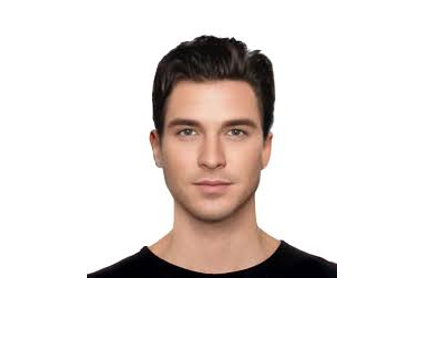
\includegraphics[scale=0.3]{imagem1.jpg}}
\subfigure[Imagem recorte\label{red2}]{
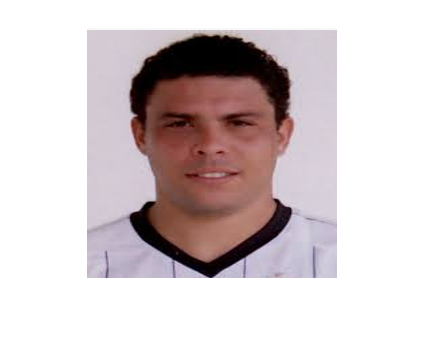
\includegraphics[scale=0.3]{imagem2.jpg}}
\end{figure}

\newline

\subsection*{Parte II}
Logo em seguida, foram detectadas as regiões de interesse (olhos, nariz e boca) e recortadas da imagem.\\


\begin{figure}[h]
\centering
\subfigure[Imagem detecção]{
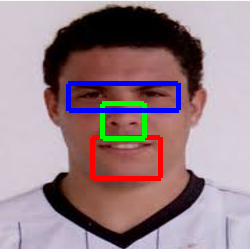
\includegraphics[scale=0.5]{deteccao.png}}
\subfigure[\label{red2}]{
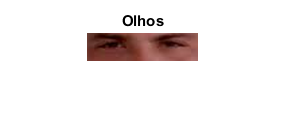
\includegraphics[scale=0.6]{olhos.png}}
\subfigure[\label{red2}]{
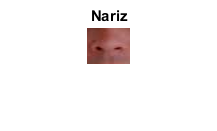
\includegraphics[scale=0.6]{nariz.png}}
\subfigure[\label{red2}]{
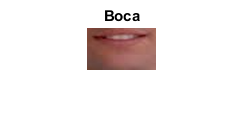
\includegraphics[scale=0.6]{boca.png}}
\end{figure}
\floatBarrier	

\subsection*{Parte III}

Posteriormente, realizou-se a detecção das posições locais de recursos e limites nos rostos detectados.

Para isso foi utilizada a função do MATLAB \textit{convhull}, função que retorna o casco convexo de um conjunto de pontos no espaço 2D ou 3D. Nesse caso, retorna o casco limitado pelos olhos, boca e nariz obtidos anteriormente. E também foi utilizada a função de detecção de bordas \textit{Sobel}.
\begin{figure}[h]
\centering
\subfigure[Convex-hull e borda]{
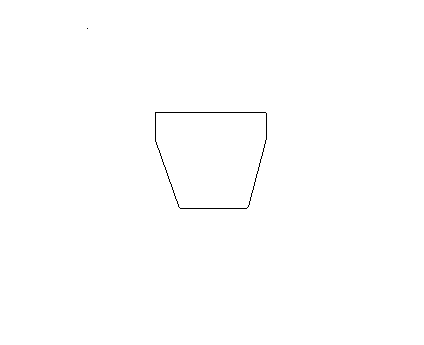
\includegraphics[scale=0.4]{borda.png}}
\subfigure[Resultado \label{red2}]{
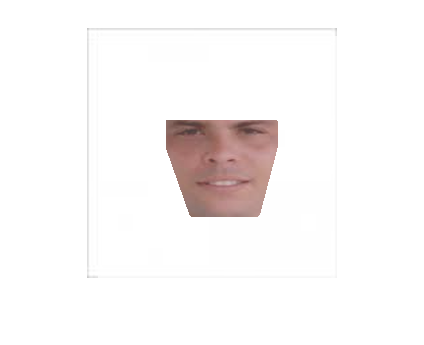
\includegraphics[scale=0.4]{covex_hull.png}}
\end{figure}

\subsection{Parte IV}

A partir das características foram criados pontos de destino para o mapeamento de um rosto para o outro, e em seguida realizou-se o redimensionamento da face recortada para o tamanho da face base, para obter um encaixe preciso desse rosto a nova face. Obtendo assim a possição exata do rosto.
Comparacao de posições:

\begin{figure}[h]
\centering
\subfigure[Posição original]{
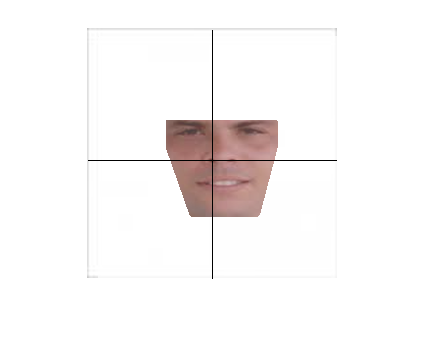
\includegraphics[scale=0.5]{posicao_original.png}}
\subfigure[Nova posicao e redimensionada \label{red2}]{
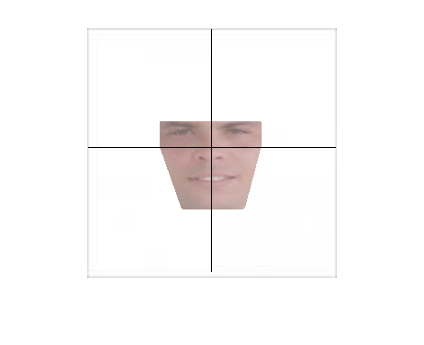
\includegraphics[scale=0.5]{nova_posicao.png}}
\end{figure}



\subsection{Parte V}

Após os procedimetos de redimencionamento e relocalização da face recortada, começou o procedimento de pigmentação da pele da face recortada.\\
Através desse procedimento tentamos aproximar-se ao máximo da cor da pele da face base para que não houvesse uma mudança de cor abrupta causando um desconforto visual. 

\begin{figure}[h]
\centering
\subfigure[Posição original]{
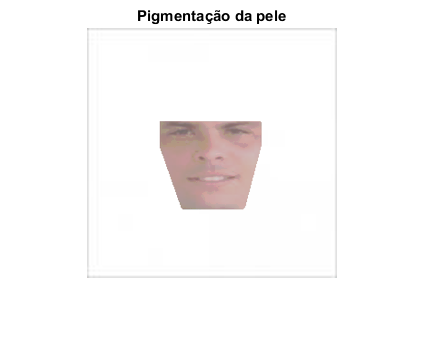
\includegraphics[scale=0.6]{pigmentacao.png}}
\end{figure}




\section{Conclusão}
A partir dos resultados obtidos, na primeira parte nota-se que a definição da morfologia bottom-hat, que destaca objetos escuros sobre um fundo claro, aplicando fechamento na imagem para obter o fundo e posteriormente subtraindo a imagem por esse fundo encontrado é afirmada. Na segunda parte, aplicando segmentação seguindo os passos instruídos, tem-se o subdivisão da imagem em objetos ou regiões como era esperado, podendo servir para diversas aplicações que necessitam dos objetos isolados. E, por fim, um vídeo YUV é lido a partir dos parâmetros solicitados, e são recuperados frames especificos nessa função e aplica-se o algoritmo de Block Matching para estimação do movimento que foi claramente aplicado.

\begin{thebibliography}{1}

\bibitem{IEEEhowto:kopka}

http://scholar.harvard.edu/stanleychan/software/subpixel-motion-estimation-without-interpolation

Materiais da disciplina

\end{thebibliography}




\end{document}


